\documentclass[letterpaper,12pt]{article}
\usepackage[utf8]{inputenc}
\usepackage[T1]{fontenc}
\usepackage[spanish]{babel}
\usepackage{graphicx, float, subcaption, anysize}
\usepackage{hyperref}
\usepackage{listings}

\usepackage{xcolor}

\renewcommand\thesection{\arabic{section}}
\marginsize{1cm}{1cm}{1cm}{1cm}

\definecolor{codegreen}{rgb}{0,0.6,0}

\definecolor{codegray}{rgb}{0.5,0.5,0.5}

\definecolor{codepurple}{rgb}{0.58,0,0.82}

\definecolor{backcolour}{rgb}{0.95,0.95,0.92}

\lstdefinestyle{mystyle}{
	backgroundcolor=\color{backcolour},   
	commentstyle=\color{codegreen},
	keywordstyle=\color{magenta},
	numberstyle=\tiny\color{codegray},
	stringstyle=\color{codepurple},
	basicstyle=\ttfamily\footnotesize,
	breakatwhitespace=false,         
	breaklines=true,                 
	captionpos=b,                    
	keepspaces=true,                 
	numbers=left,                    
	numbersep=5pt,                  
	showspaces=false,                
	showstringspaces=false,
	showtabs=false,                  
	tabsize=2
}

\lstset{style=mystyle}

\lstset{
literate={ó}{{\"o}}1
{á}{{\"a}}1
{ú}{{\"u}}1
{é}{{\"u}}1
{í}{{\"u}}1
}



\begin{document}
	\begin{figure}
		\subfloat{
\includegraphics[width = 0.2\textwidth]{img/unamescudo}}
		\hfill
		\subfloat{
\includegraphics[width = 0.2\textwidth]{img/escudofi_negro}}
	\end{figure}

	\begin{titlepage}
		\centering
		{\bfseries\LARGE UNIVERSIDAD NACIONAL AUT\'ONOMA DE M\'EXICO \par}
		\vspace{1cm}
		{\bfseries\LARGE FACULTAD DE INGENER\'IA \par}
		\vspace{1cm}
		{\itshape\Large\textbf{Asignatura: Bases de Datos (1644)}\par}
		\vspace{1cm}
		{\itshape\Large\textbf{Documentación Proyecto final.}\par}
		\vspace{1cm}
		{\itshape\Large \textbf{Profesor: Ing. Fernando Arreola Franco}
			\par}
		\vspace{1cm}
		\vfill
		{\itshape\Large \textbf{Integrantes del equipo:}\\\par}

		\begin{itemize}

			\centering

			{\itshape\Large

				\item [\textbullet] Bautista P\'erez Brian Jassiel

				\item [\textbullet] Guzmán Ramírez Aldo Yael
				\item [\textbullet] Pacheco Salgado Mauricio
				\item [\textbullet] Romero Rivera Geovanni
				\item [\textbullet] Vargas Jordán Antonio}

		\end{itemize}
		\vfill
		{\itshape\Large Grupo: 01\par}
		{\itshape\Large \textbf{Semestre: 2022-1}\par}
		{\itshape\Large \textbf{Fecha de entrega: \today}\par}
	\end{titlepage}

	\tableofcontents
	\newpage
	
	\section{Introducción}
	Durante este proyecto haremos el diseño de una página web en donde el usuario podrá realizar las compras de papelería. El frontend fue realizado en HTML y CSS y para el backend utilizamos el framework de PHP Laravel. Para el almacenamiento de datos utilizamos el lenguaje SQL con ayuda del DBMS PostgreSQL.
	En esta lo primero que debe realizarse será el registro por parte del usuario para tener sus datos almacenados para posteriormente pueda realizar sus compras y que éstas sean almacenadas para que proceda a hacer el pago de sus productos. 
	Lo que nuestra base almacenara será el nombre del usuario, así como una clave con la cual se pueda identificar si en otra ocasión decide volver a comprar. También ser hará el registro de los productos que realice, así como la fecha, total de productos que se llevó y el total a pagar. Esto para mantener un registro en nuestra venta de nuestros productos.
	Podrán hacer consultas de la cantidad de productos vendidos, así como el ingreso total de ventas en un lapso dado. También podrá ver informe de los productos que quedan en el inventario.
	
	\section{Objetivos}
	\begin{itemize}
		\item Se realizará la creación de una página web en la cual puedan realizarse compras de artículos de papelería.
		\item Usar una base de datos en la cual se almacenará la información necesaria para dicha página.
		\item Comprender el manejo de información entre la página web y la base de datos.
		\item Hacer uso de PL / SQL.
	\end{itemize}
	
	\section{Plan de trabajo}
	
	La organización de todo el proyecto requirió de sesiones semanales o bien cada tercer día dependiendo de la disponibilidad de todos los integrantes. En una primera instancia se realizó este diagrama de Gantt con la intención de dividir este proyecto por fases, quedando de la siguiente forma:
	
	\begin{figure}[H]

		\begin{subfigure}{20cm}

			\centering

			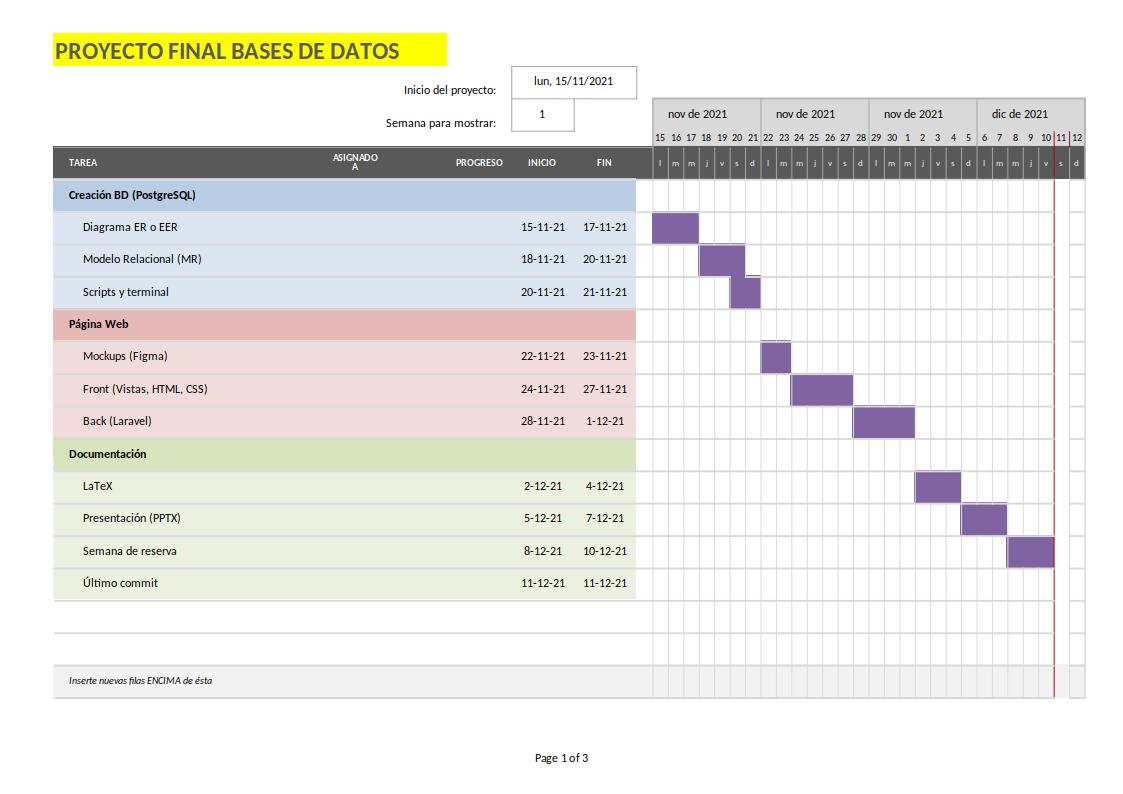
\includegraphics[width=0.9\textwidth]{img/Gantt_ProyectoBD.jpg}

		\end{subfigure}

	\caption{Diagrama de Gantt del proyecto.}
	\end{figure}
	
	\section{Diseño}
	
	Se cubrieron tres rubros importantes: El diseño conceptual y lógico de la base de datos junto con su implementación en terminal, luego el diseño de la página web en el cual se realizó tanto frontend como backend y finalmente la realización de la documentación. \\
	
	Cada parte se realizó conforme a la planeación realizada previamente, en la primera semana tocó cubrir la creación de la base de datos, en la cual se  obtuvo el modelo entidad relación y el modelo relacional, posteriormente se crearon las vistas para la página tales como el inicio, el login, el register, la sección de las compras y el catálogo y después se creó el proyecto de Laravel para programar ya toda la página y conectarla a la base de datos.
	
	
	\section{Implementación}
	
	Como primer paso para el diseño de nuestra base de datos creamos un diagrama entidad relación en el que se crearon 3 entidades principales sobre las que se trabajo todo el proyecto, estas son: “CLIENTES”, “INVENTARIO” y “PROVEEDORES”. Consideramos que son las únicas entidades necesarias, ya que otros aspectos como la compra de producto o la venta a los clientes se pueden detallar mediante la relación entre estas.
	
	\begin{figure}[H]

		\begin{subfigure}{20cm}

			\centering

			\includegraphics[width=0.9\textwidth]{/home/brian/Documentos/proyecto_bd/Diagramas/Entidad-Relación.png}

		\end{subfigure}

		\caption{Diagrama de Entidad Relación.}
	\end{figure}

 	Una vez definido eso se paso al mapeo intermedio y el diagrama relacional, en el cual definimos los tipos de datos e importancia de cada atributo, así como la cardinalidad final y paso de llaves foráneas.
 	
 	\begin{figure}[H]

 		\begin{subfigure}{20cm}

 			\centering

 			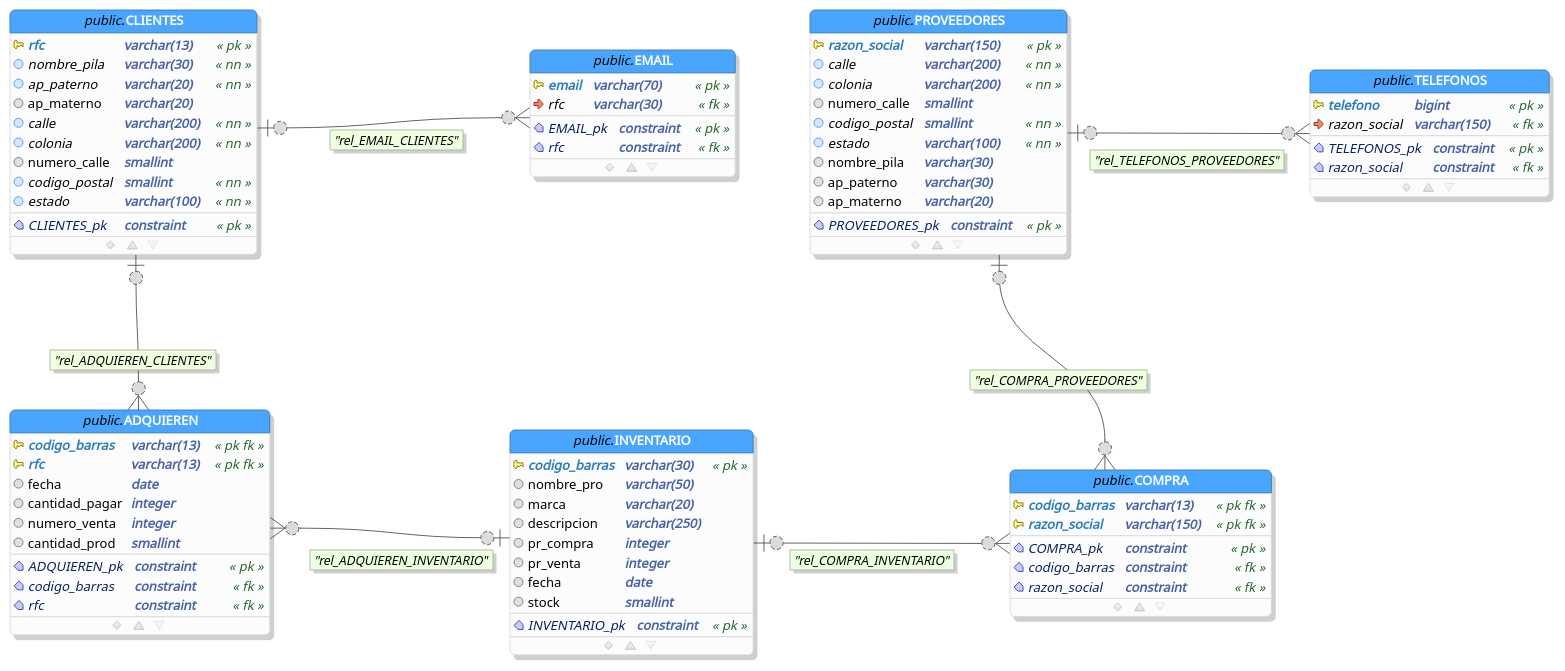
\includegraphics[width=0.9\textwidth]{//home/brian/Documentos/proyecto_bd/Diagramas/Relacional}

 		\end{subfigure}

 		\caption{Modelo Relacional.}
 	\end{figure}
 
 	Creamos la base de datos
 	
 	\lstinputlisting[language=SQL, firstline=12, lastline=12]{/home/brian/Documentos/proyecto_bd/Script/scriptbd.sql}

 	
 	Creamos una secuencia en donde el mínimo valor sea 0 y el máximo sea 100 donde sec\_ad se vaya incrementando uno en uno.
 	
 	\lstinputlisting[language=SQL, firstline=15, lastline=22]{/home/brian/Documentos/proyecto_bd/Script/scriptbd.sql}
 	
 	cCreamos una tabla publica llamada clientes con 9 atributos con sus respectivos datos: varchar y smallint, utilizamos constraint en donde seleccionamos que el campo rfc tiene que ser único y para ello lo seleccionamos como llave primaria.
 	y en la mayoría de los atributos los designamos not null para que no queden vacíos.
 	
 	\lstinputlisting[language=SQL, firstline=33, lastline=45]{/home/brian/Documentos/proyecto_bd/Script/scriptbd.sql}
 	
 	Con el alter table y el owner to, cambiamos de propietario de la base de datos siendo postgres como su propietario.

 	\lstinputlisting[language=SQL, firstline=47, lastline=47]{/home/brian/Documentos/proyecto_bd/Script/scriptbd.sql}
	
	Creamos una tabla publica llamada email con 2 atributos con sus datos varchar, siendo su llave primaria email utilizando constraint para su unicidad.\\
	
	\lstinputlisting[language=SQL, firstline=52, lastline=57]{/home/brian/Documentos/proyecto_bd/Script/scriptbd.sql}
	
	con el alter table y el owner to, cambiamos de propietario a la tabla publica email siendo postgres como su propietario
	
	\lstinputlisting[language=SQL, firstline=59, lastline=59]{/home/brian/Documentos/proyecto_bd/Script/scriptbd.sql}
	
	Creamos una tabla publica llamada adquieren con 6 atributos con sus respectivos datos: varchar, dar, smaillint y float, en donde es una relacion de m:m entre las tablas clientes e inventario teniendo como llave primaria compuesta el codigo de barras y el rfc.
	En el atributo numero\_venta designamos una restriccion llamada default, el cual nos permite colocar un dato por defecto seguido de un nextval que nos va a servir.
	Para recuperar los valores de una secuencia y en este caso la secuencia es la que creamos anteriormente "sec\_ad" el cual va aumentando de 1 en 1 hasta 100 a medida que se ingrese el número de venta.
	y designando not null en algunos atributos.
	
	\lstinputlisting[language=SQL, firstline=64, lastline=73]{/home/brian/Documentos/proyecto_bd/Script/scriptbd.sql}
	
	Cambiamos de propietario a la tabla pública email.
	
	\lstinputlisting[language=SQL, firstline=75, lastline=75]{/home/brian/Documentos/proyecto_bd/Script/scriptbd.sql}
	
	Creamos la tabla pública inventario con 8 atributos con sus respectivos datos varchar, float, date, smallint asignado como llave primaria codigo\_barras.
	
	\lstinputlisting[language=SQL, firstline=80, lastline=91]{/home/brian/Documentos/proyecto_bd/Script/scriptbd.sql}
	
	Cambiamos de propietario a la tabla pública inventario.
	
	\lstinputlisting[language=SQL, firstline=93, lastline=93]{/home/brian/Documentos/proyecto_bd/Script/scriptbd.sql}
	
	Creamos la tabla publica llamada compra con 2 atributos con sus datos varchar siendo estos not null.
	Al ser una relación m:m entre las tablas inventario y proveedores, vamos a tener una llave primaria compuesta con sus respectivas llaves primarias: codigo\_barras y razon\_social.
	
	\lstinputlisting[language=SQL, firstline=98, lastline=103]{/home/brian/Documentos/proyecto_bd/Script/scriptbd.sql}
	
	Cambiamos de propietario a la tabla pública compra:
	
	\lstinputlisting[language=SQL, firstline=105, lastline=105]{/home/brian/Documentos/proyecto_bd/Script/scriptbd.sql}
	
	Creamos la tabla publica proveedores con 9 atributos con sus respectivos datos: varchar, small int y integer siendo algunos de estos not null, asignando como llave primaria la razon social
	
	\lstinputlisting[language=SQL, firstline=110, lastline=122]{/home/brian/Documentos/proyecto_bd/Script/scriptbd.sql}
	
	Cambiamos de propietario a la tabla pública proveedores.
	
	\lstinputlisting[language=SQL, firstline=124, lastline=124]{/home/brian/Documentos/proyecto_bd/Script/scriptbd.sql}
	
	Creamos la tabla pública llamada teléfonos con 2 atributos con sus respectivos datos: varchar y bigint, y asignamos la llave primaria teléfono.
	
	\lstinputlisting[language=SQL, firstline=129, lastline=134]{/home/brian/Documentos/proyecto_bd/Script/scriptbd.sql}
	
	Cambiamos de propietario a la tabla a la tabla pública teléfonos.
	
	\lstinputlisting[language=SQL, firstline=136, lastline=136]{/home/brian/Documentos/proyecto_bd/Script/scriptbd.sql}
	
	Con alter table modificamos la tabla email añadiendo una restricción de llave foránea siendo el atributo rfc y a la vez esta referenciado a la tabla clientes.
	La última sentencia se refiere a que, si en algún momento se elimina o se mejora una fila de la tabla principal, no va a realizar ninguna acción y va a devolver un error “evita eliminar un padre cuando hay hijos”.
	
	\lstinputlisting[language=SQL, firstline=141, lastline=143]{/home/brian/Documentos/proyecto_bd/Script/scriptbd.sql}
	
	Modificamos la tabla adquieren añadiendo una llave foránea llamada codigo\_barras de la tabla inventario. \\
	Y si en dado caso se eliminara una fila de la tabla principal va a devolver un error.
	
	\lstinputlisting[language=SQL, firstline=148, lastline=150]{/home/brian/Documentos/proyecto_bd/Script/scriptbd.sql}
	
	Modificamos la tabla adquieren añadiendo otra llave foránea llamada rfc de la tabla clientes.
	Recordemos que la tabla adquiere es una relación entre esas dos tablas y su llave primaria es una llave compuesta entre las dos llaves primarias de las dos tablas.
	Poniendo la misma sentencia de que si se modifica algo incorrecto en la tabla principal, no hará nada y devolverá un error.
	
	\lstinputlisting[language=SQL, firstline=162, lastline=164]{/home/brian/Documentos/proyecto_bd/Script/scriptbd.sql}
	
	La tabla compra es una relación entre las tablas inventario y proveedores entonces le agregamos otra llave foránea llamada razon\_social de la tabla proveedores.
	Poniendo la misma sentencia de que si se modifica algo incorrecto en la tabla principal, no hará nada y devolverá un error
	
	
	\lstinputlisting[language=SQL, firstline=169, lastline=171]{/home/brian/Documentos/proyecto_bd/Script/scriptbd.sql}
	
	Modificamos la tabla teléfonos añadiéndole una llave foránea llamada razon\_social de la tabla proveedores.
	Poniendo la misma sentencia de que si se modifica algo incorrecto en la tabla principal, no hará nada y devolverá un error.
	
	\lstinputlisting[language=SQL, firstline=176, lastline=178]{/home/brian/Documentos/proyecto_bd/Script/scriptbd.sql}
	
	Posterior a esto, procederemos a insertar los datos (Las inserciones no so mostrarán en este documento para no extender este documento, sin embargo, todas las inserciones están en el script)
	
	Posterior a las inserciones se crearán las funciones PL/SQL en las que desarrollamos las tareas solicitadas, por ejemplo, el primer punto pedía que a través del código de barras de un producto nos regresara la utilidad, lo que interpretamos como mostrar el nombre, descripción y precio de un producto. Cosa que logramos mediante un “RETURN QUERY SELECT” dentro de una función como se muestra a continuación.
	
	\lstinputlisting[language=SQL, firstline=251, lastline=258]{/home/brian/Documentos/proyecto_bd/Script/scriptbd.sql} 
	
	Lo que regresamos es una tabla con los atributos mencionados, y tal como podría haber sido de manera normal, solo tenemos que crear una consulta siendo específicos sobre lo que nos interesa encontrar. 
	Finalmente, podemos observar como funciona 
	
	
	\begin{figure}[H]

		\begin{subfigure}{20cm}

			\centering

			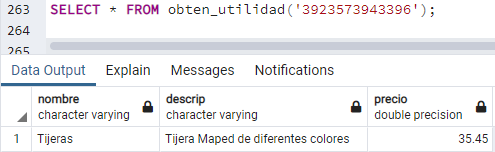
\includegraphics[width=0.9\textwidth]{img/01}

		\end{subfigure}

	\end{figure}

	Este fue un proceso que repetimos bastante, ya que la mayoría de los puntos se resolvían con consultas, por lo que solo teníamos que ingeniarnos una manera de acomodar los datos y los atributos de manera que cumplieran nuestros requisitos, por ejemplo, el caso de obtener productos de los cuales solo quedaran menos de 3 en stock.
	
		\lstinputlisting[language=SQL, firstline=264, lastline=273]{/home/brian/Documentos/proyecto_bd/Script/scriptbd.sql}
		
	Este tipo de ejercicios nos resultaron bastante útiles, pues de esta manera practicamos usando diversas herramientas de consulta y filtrado de datos, como el “GROUP BY” o “HAVING”
	
	\begin{figure}[H]

		\begin{subfigure}{20cm}

			\centering

			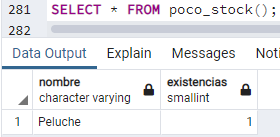
\includegraphics[width=0.9\textwidth]{img/02}

		\end{subfigure}

	\end{figure}
	
	Para el punto donde teníamos que ingresar una o dos fechas y teníamos que obtener el total de artículos vendidos más la ganancia obtenida en ese periodo o fecha, presento un pequeño reto pues se tenía la intención de crear una única función que fuera capaz de aceptar uno o dos fechas como parámetros, sin embargo optamos  por crear dos funciones con el mismo nombre, que fueran llamadas según los parámetros que se proporcionaran al ejecutarlas, tal como vimos un poco en una de las clases de teoría; obteniendo lo siguiente
	
	\lstinputlisting[language=SQL, firstline=281, lastline=300]{/home/brian/Documentos/proyecto_bd/Script/scriptbd.sql}
	
	Como observamos, ambas funciones son exactamente la misma, con la diferencia como ya se mencionaba, de contar con un parámetro menos para así poder obtener la venta y ganancia de una única fecha dada, a continuación, una muestra del funcionamiento de ambas, y para que se puedan comprobar los resultados, se va a proveer la información registrada de dos ventas.
	
	
	\begin{figure}[H]

		\begin{subfigure}{20cm}

			\centering

			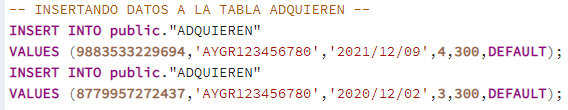
\includegraphics[width=0.9\textwidth]{img/03}

		\end{subfigure}

	\end{figure}

	Como se ve, el 9 de diciembre de 2021 hubo una venta de 4 artículos por un precio de 300 pesos totales, y el 2 de diciembre de 2020 se vendieron 3 artículos por un precio total de 300 pesos también
	Ahora veamos que arrojan nuestras funciones
	
	\begin{figure}[H]

		\begin{subfigure}{20cm}

			\centering

			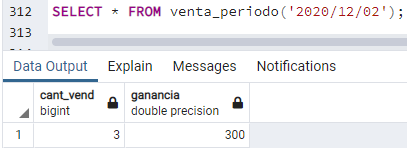
\includegraphics[width=0.9\textwidth]{img/04}

		\end{subfigure}

	\end{figure}
	
	Pues bien, tenemos precisamente lo que esperábamos, dada la fecha del 2 de diciembre de 2020 hubo una venta total de 3 artículos con un precio total de 300 pesos 
	
	\begin{figure}[H]

		\begin{subfigure}{20cm}

			\centering

			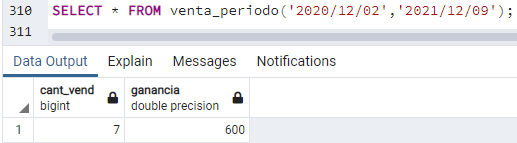
\includegraphics[width=0.9\textwidth]{img/05}

		\end{subfigure}

	\end{figure}
	
	Finalmente, durante el periodo de las dos fechas, tenemos la venta de 7 artículos con una ganancia de 600 pesos
	
	\begin{figure}[H]

		\begin{subfigure}{20cm}

			\centering

			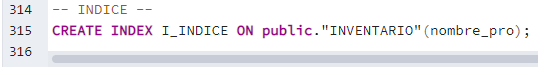
\includegraphics[width=0.9\textwidth]{img/06}

		\end{subfigure}

	\end{figure}

	Finalmente, como se pedía hemos creado un índice dentro de la tabla inventario y sobre la columna nombre, pues es una de las más consultadas y mediante éste podemos asegurarnos de tener consultas más rápidas y eficientes. 
	
	
	
	\section{Presentación}
	
	\textbf{Página web}
	
	Para conectar la página web a la base de datos se hizo el uso de Laravel, el cual es un framework de PHP que se puede integrar perfectamente con PostgreSQL y otros manejadores como MySQL, MariaDB, etc.
	
	El procedimiento para instalar Laravel es el siguiente:
	
	\begin{itemize}
		\item Instalar PHP
		\item Instalar NodeJS (de preferencia una versión mayor a la 12)
		\item Instalar Composer que es el que hace posible la creación del proyecto
	\end{itemize}

	
	Al crear un proyecto en Laravel se crean diferentes archivos entre los cuales tenemos uno llamado .env, en dicho archivo se modifican los parámetros del proyecto tal como se muestra a continuación:
	
	\begin{figure}[H]

		\begin{subfigure}{20cm}

			\centering

			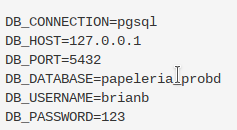
\includegraphics[width=0.9\textwidth]{img/v7}

		\end{subfigure}

	\end{figure}

	Una vez creado el proyecto se integrará todo con las vistas creadas. (Este proceso se explicará en la presentación)
	
	Esta ventana es nuestra vista principal en la cual podemos observar una bienvenida, así como una barra de menú en la cual están las opciones de inicio, iniciar sesión y crear cuenta.
	
	\begin{figure}[H]

		\begin{subfigure}{20cm}

			\centering

			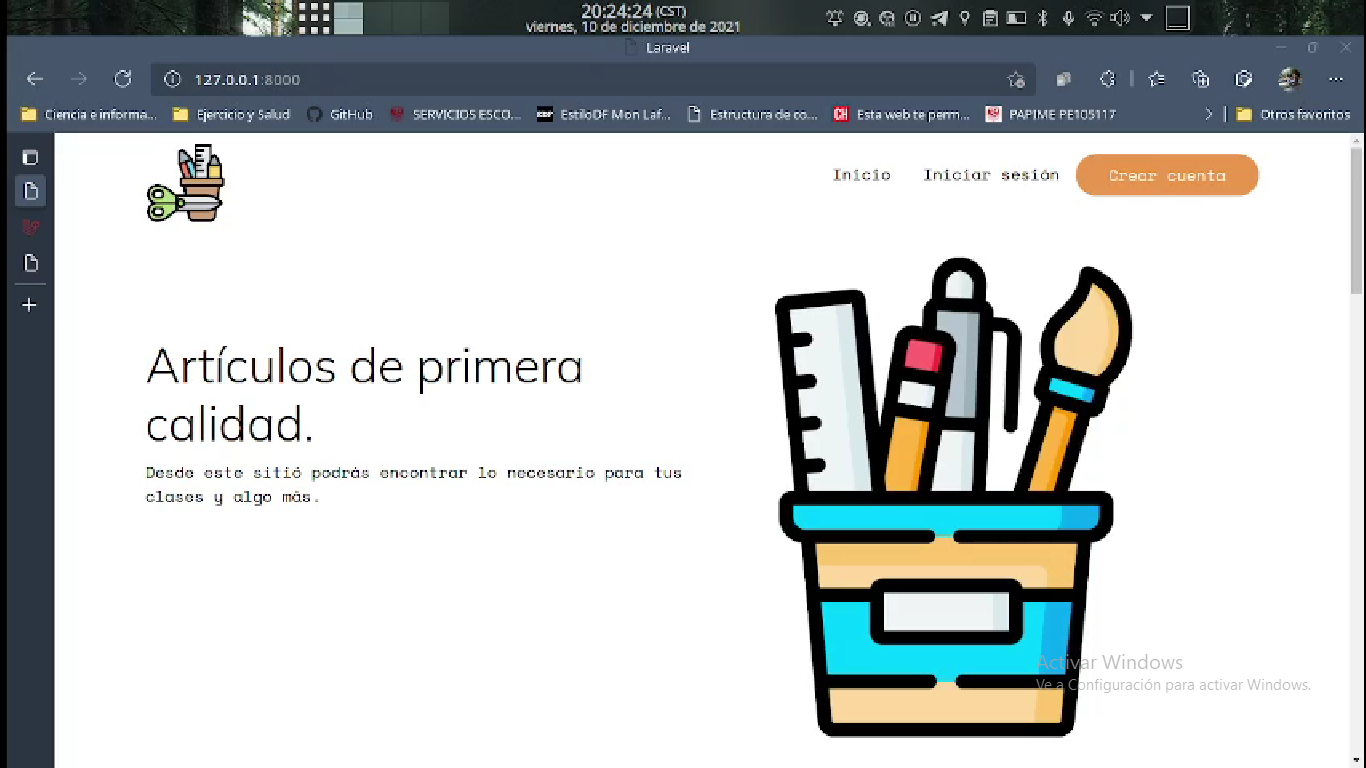
\includegraphics[width=0.9\textwidth]{img/v1}

		\end{subfigure}

	\end{figure}

	Si nos deslizamos hacia abajo, nos aparecerán los productos que deseemos comprar, si queremos añadirlos a nuestro carrito aun no podremos ya que tendremos que registrarnos primero.
	
	\begin{figure}[H]

		\begin{subfigure}{20cm}

			\centering

			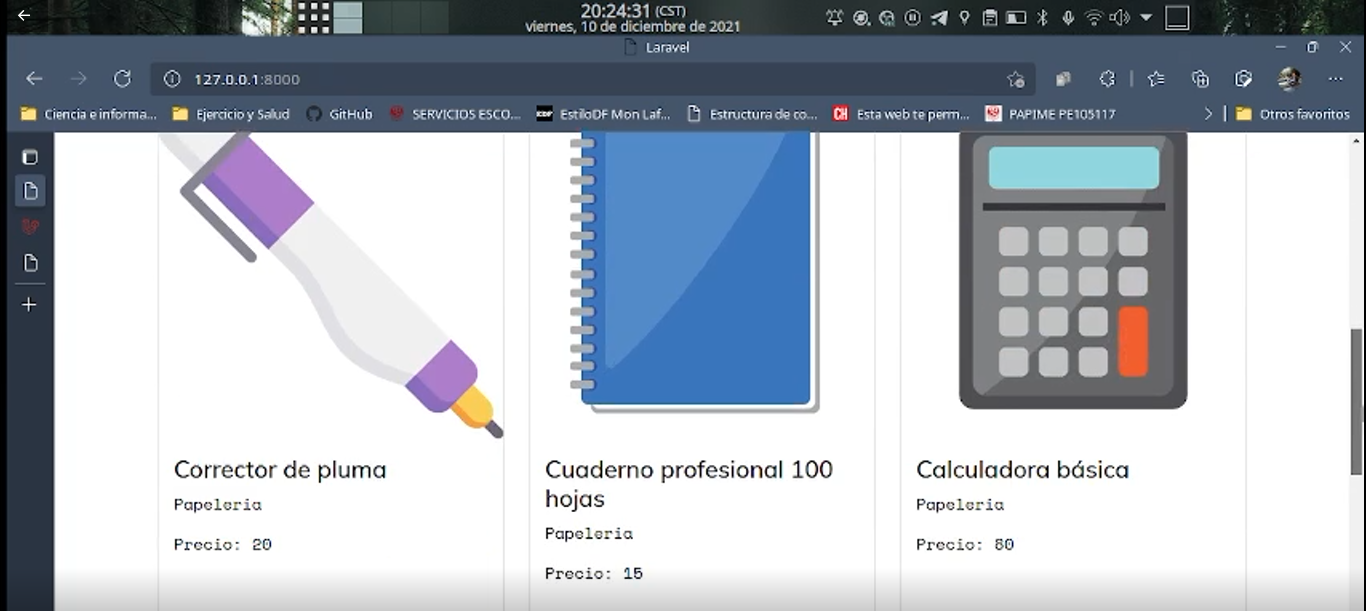
\includegraphics[width=0.9\textwidth]{img/v2}

		\end{subfigure}

	\end{figure}

	Así que si le damos clic nos mandara a la parte de iniciar sesión.
	
	\begin{figure}[H]

		\begin{subfigure}{20cm}

			\centering

			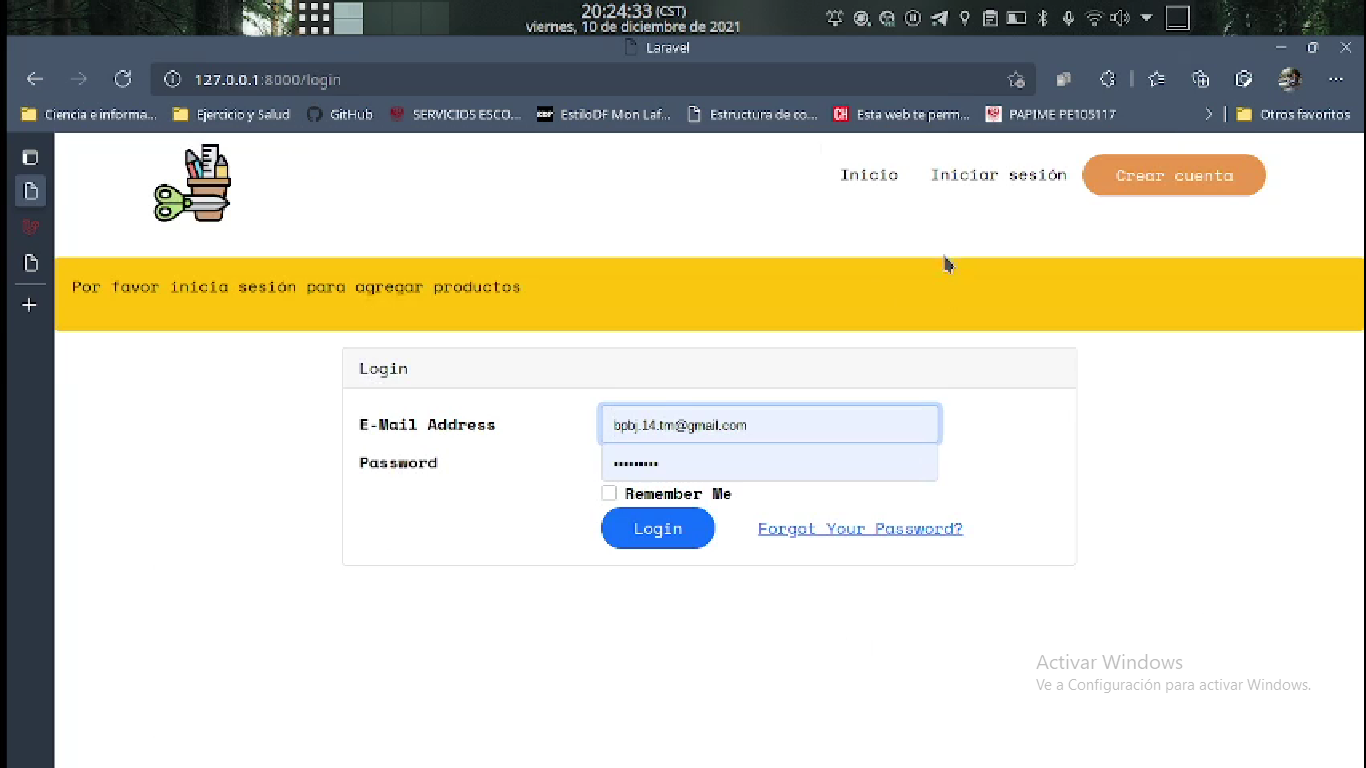
\includegraphics[width=0.9\textwidth]{img/v3}

		\end{subfigure}

	\end{figure}

	Una vez iniciando sesión el producto estará registrado en nuestro carrito de compras
	
	\begin{figure}[H]

		\begin{subfigure}{20cm}

			\centering

			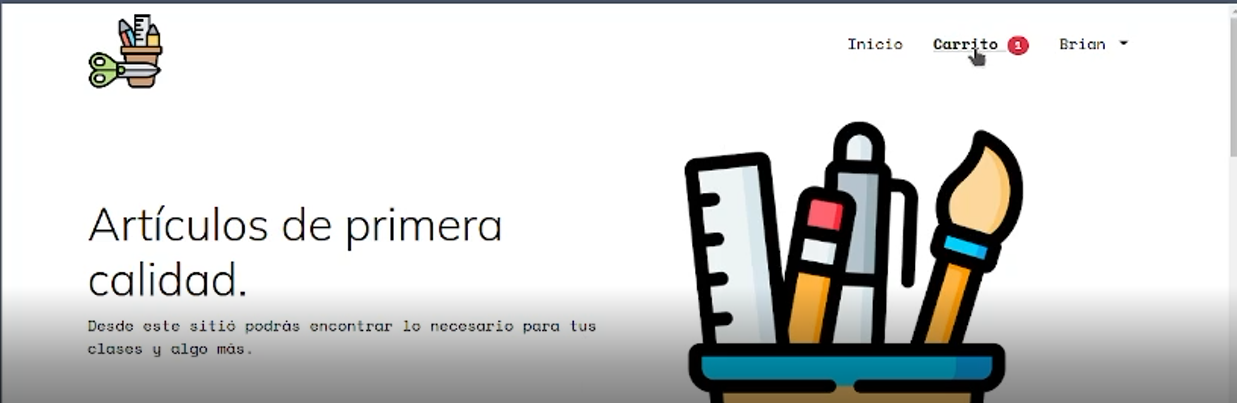
\includegraphics[width=0.9\textwidth]{img/v4}

		\end{subfigure}

	\end{figure}

	Vamos a esta vista:
	En este espacio podemos observar las siguientes características del producto tales como:
	
	\begin{itemize}
		\item Nombre del producto.
		\item Precio.
		\item Cantidad.
		\item Subtotal.
	\end{itemize}

	\begin{figure}[H]

		\begin{subfigure}{20cm}

			\centering

			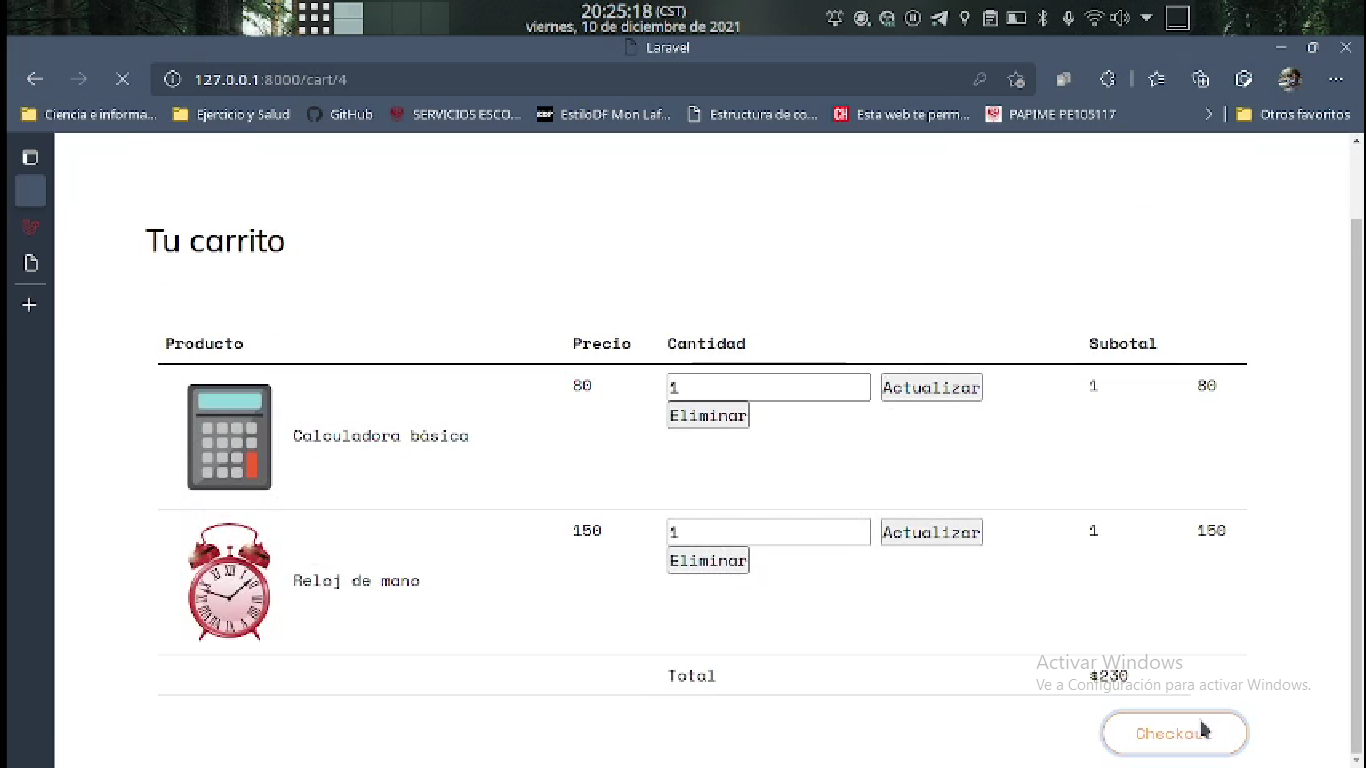
\includegraphics[width=0.9\textwidth]{img/v5}

		\end{subfigure}

	\end{figure}

Y al hacer checkout se mostrará la factura de compra.

\begin{figure}[H]

	\begin{subfigure}{20cm}

		\centering

		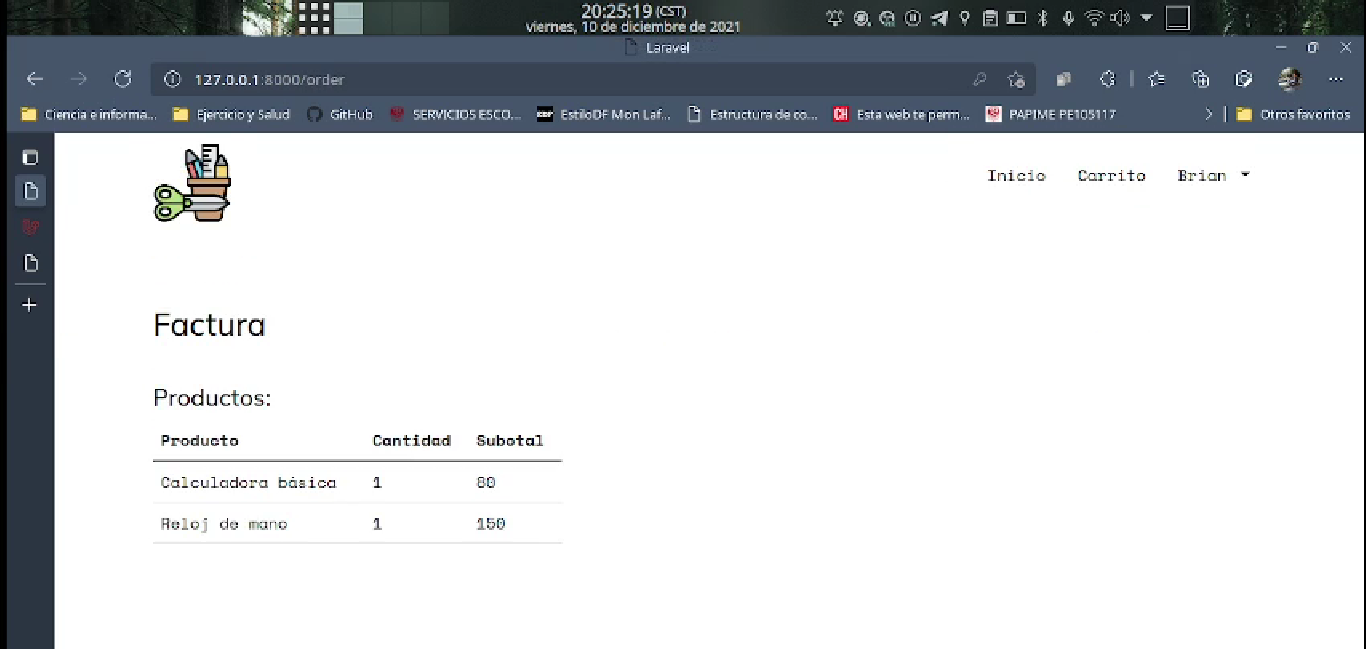
\includegraphics[width=0.9\textwidth]{img/v6}

	\end{subfigure}

\end{figure}
	
	\section{Conclusiones}
	\begin{itemize}
		\item Brian Bautista: Respecto al proyecto, debo decir que fue un gran reto dado que sí fueron varios requerimientos y uno de ellos fue externo a lo que se vio en clase, sin embargo, no fue problema dado a que yo ya tenía un poco de experiencia utilizando Laravel, lo cual nos ahorró tiempo para crear la página. Debo decir que quedo satisfecho dado que mayormente el proyecto quedo tanto a nivel PL / SQL como en la página, aunque en este último rubro tuvimos problemas para cubrir al cien por ciento la parte de las compras ya que sí podemos insertar productos y simular la compra, sin embargo el stock no decrementó en la página. Aún así creo que para ser un primer proyecto grande en Laravel quedó muy bien. 
		\item Aldo Guzmán:
		Como modo de aprendizaje me llevo la experiencia de realizar la base de datos implementado a la página web. Así como empezar a crear funciones, triggers. Lo más pesado fue ingeniarse las funciones de tal forma que nosotros manipulemos la información para lograr lo requerido, así como la unión entre la base y la página. A pesar de que no logramos algunos puntos requeridos, gracias a todos mis compañeros de equipo realizamos la investigación para realizar la mayor parte de estos. Fue un proyecto realmente bueno el tiempo logro sobrepasarnos, así como también algunos conocimientos de programación que no logramos aprender con el tiempo. Pero nos quedamos con la experiencia de como organizarnos en un ámbito profesional y saber designar los roles para que cada miembro se centre en lo que mejor sabe hacer.
		\item Mauricio Salgado:
		Durante la realización de este proyecto tuvimos ciertas formas dudas y tuvimos que investigar algunas consultas previas que se nos complicaron a la hora de la programación de la base de datos. Fuera de esto, podemos decir que se cumplieron la mayoría de los puntos del proyecto, es un proyecto sencillo pero demandante, por lo que el trabajo en equipo fue esencial para que saliera todo bien y teniendo un orden para la realización de incluso la programación de las páginas web y los esquemas de entidad relación. Podemos decir que es un proyecto que nos adentra a lo que puede ser un ejercicio que nos adentra al campo laboral y que nos puede ayudar de referencia en futuros proyectos, por lo que es necesario saber entender en todo momento es un proyecto que contiene la mayoría del curso impartidos durante el semestre.
		\item Geovanni Romero:
		El proyecto fue de gran nivel y comenzamos a investigar desde cómo realizar una página web tanto el back end y front end. La parte que más me favoreció fue al momento de crear las funciones y los triggers. Mis compañeros de equipo supieron apreciar esto y me puse a trabajar en ello. La organización que tuvimos fue bastante buena debido a que todos colaborábamos en todo momento desde que iniciamos creando los modelos entidad relación y el relacional hasta la unión entre la base y la página. A la hora de programar funciones e implementar ciertas consultas en la base de datos, tuve que ingeniármelas con mis conocimientos previos obtenidos en el curso, era un poco confuso al inicio, pero una vez identificando los errores o mejor dicho la forma correcta de codificar en la base respetando la sintaxis y verificando que algunas palabras no fueran sensibles al lenguaje durante de esto. Todo fue más fácil después, por lo que en ciertos puntos eran un poco más sencillos de comprender que otros, o por lo menos unos tenían cierta dificultad personal. Pero nada que no se pueda realizar complementando conocimientos con mis compañeros de equipo e indagando un poco en lo que es la programación web implementada a las bases de datos desde postgres. Incluso puedo decir que algunos puntos eran complejos no por su dificultad, si no que en lo personal no había cierta información para implementarla en la web o en ciertos libros consultados para la parte de PL/SQL.
		\item Antonio Vargas:
		Fue uno de los proyectos mas interesantes y completos que he realizado durante todo mi transcurso en la Facultad porque a la hora de realizarlo se me presentaron distintas dificultades que sabia que tarde o temprano iban a presentarse como un reto si quería seguir adelante como estudiante de Ingeniería. 
		Uno de los retos fue a la hora de realizar una pagina web, añadiendo un index.html y su css. Diría que fue una de las partes más difíciles para mí, porque no tenía tantas bases y no sabía cómo realizarla, pero al final, viendo videos y buscando información sobre html y css se logró, y puedo decir que no fue tan difícil como pensaba y sobre todo es interesante y entretenido crear paginas a tu gusto. 
		Otro de los retos a la hora de programación fue cumplir de manera exitosa los puntos de la Parte Uno ya que tuvimos que recordar lo visto de las clases pasadas, revisar los apuntes y ver de nuevo las clases y nos llevo más tiempo de lo previsto, pero aun que los puntos estuvieron complejos al principio se logró programar casi todo lo requerido ya que nos faltó que el stock decrementara por cada venta de ese artículo.    
		Aunque se presentaron otros retos con menor dificultad, como enlazar todas las paginas que realizo el equipo o la forma en como conectar la Pagina a una base de datos, etc. Se cumplieron las expectativas del Proyecto, ya que al realizar la Pagina con ciertos requerimientos, así como tener toda su base de datos hizo que todo el equipo tuviera más conocimiento y más experiencia con el manejo de las Paginas conectadas a una base de datos.
		Me siento bastante satisfecho llegar al final de esto, hicimos una pagina de una Papeleria que cuenta con su sistema de login, creación de cuenta, carrito, factura y artículos de papeleria. En donde el usuario puede registrarse y así poder comprar distintos artículos y ser consciente de los productos que tiene en el carrito, así como tener a su dirección de envio y del lado del Dueño, tener control sobre que usuario se registra, que compra y cuanto compra, también tener acceso al stock de cada articulo y saber cuando contactar con los proveedores, pero sobre todo se logro de manera exitosa aplicar los conceptos vistos en clase. 
		Hubo muchas gotas de sudor, muchas neuronas quemadas, muchas lágrimas, pero por fin el proyecto está terminado.
	\end{itemize}
	
\end{document}